\normalfont\normalsize
\chapter{Software Implementation}

In this chapter we will present a simple yet efficient scheduling algorithm for single hop networks.

State-of-the-art algorithms require to measure the consumed energy in other to dynamically schedule transmission
task. This is not very desirable in real world, where a lot of variables can generate a big error in the estimated energy left

\begin{itemize}
    \item Large changes in temperature can alter the total energy stored
    \item Leakage currents, that can vary between charges and different levels of stored energy
    \item Differences between supposed identical super-capacitors.
\end{itemize}

In order to simply the algorithms for the user to deploy it faster in a real EHWSN applications,
we have implemented and tested a simple dynamic scheduling algorithm for transfered data.

The algorithm can be considered to have very basic water-filling policy, with one slot that is
the current discharge period. This simplifies the implementation and reduces the computational
requirements. It is designed to be run with an energy harvesting module that has a super capacitor
as energy storage unit. Because of this, we simplified the predictor in order to obtain O(1)
complexity.

The capacitor does not discharge very linear, but in the tests we have conducted, the error is
small enough to allow us to estimated de remaining time without the requirement of measuring how
much energy did the capacitor stored and how much energy is was consumed.

\begin{figure}[ht] \centering
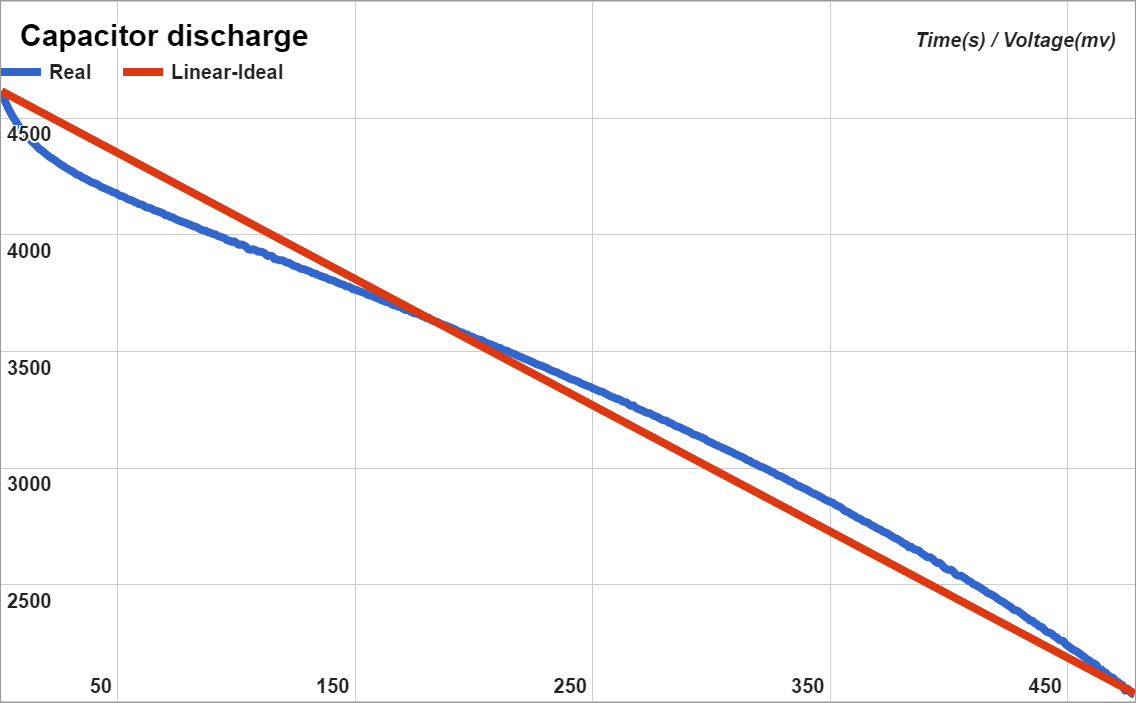
\includegraphics[width=0.85\textwidth]{img/capacitor.png}
\caption{1F EDLC capacitor discharge}
\end{figure}


\newcommand{\var}[1]{{\ttfamily#1}}% variable
\begin{algorithm}[t]
  \caption{Send frequency scheduling Algorithm}\label{euclid}
  \begin{algorithmic}[1]
    \Procedure{algorithm}{$voltage,time$}\Comment{}
    \State determine current state Charging/Discharging
    \If{changed from Charging to Discharging}
        \State Calculate the new target time
        \State Calculate the frequency based on total number of sent data
        \State $changedVoltage \gets voltage$
    \EndIf
    \If{current state is Discharging}
    \If{$voltage < MIN\_COMPUTE\_DELTA$}
        \State $sendFreq \gets sendFreq / 2$
    \EndIf
    \State $deltaVoltage \gets changedVoltage - voltage$
    \If{$deltaVoltage > MIN\_VOLTAGE\_DELTA$}
        \State Estimate the new remaining time
        \State Calculate remaining time until deadline
        \State $newSendFreq \gets sendFreq*estimated*percentagePenalty/remaining $
        \If {$newSendFreq != sendFreq$}
            \State Change the speed
            \State $changedVoltage \gets voltage$
        \EndIf
    \EndIf
    \EndIf
    \EndProcedure
  \end{algorithmic}
\end{algorithm}


The algorithm has a total time that it needs to respect, while trying to maximize the total number
of packets sent. In order to achieve this two simple requirements, it dynamically estimates the
remaining time and, according to the difference between the estimation and the remaining time, it
keeps the same send frequency or alters it. Because when lowering the speed, the total consumed
energy will not be halved, due to leakage and sleep current, a penalty is imposed,
one that we selected at 75\%. Furtermore, in order to make sure that the deadline is respected,
under a certain voltage level the
speed is halved and kept until the energy is depleted or the capacitor is recharged. Every time the
frequency changes, the interval used to compute the estimated time is updated.

The algorithm is very versatile, with many customization options, depending on the type of hardware and
requirements of the application in which it is used.

What can be changed and it is recommended to be changed is presented in the list bellow.  Other
customization options exists, but it is not recommended to changed them.

\begin{itemize}
    \item DEFAULT\_TARGET\_TIME The default deadline for the algorithm. After one iteration it is
        dynamically adjusted.
    \item TIME\_PERCENTAGE\_PENALTY Alters the estimated time by either reducing it or increasing
        it.
    \item TIME\_EXTRA\_REMAINING When computing the new frequency, this is added to the remaining
        time in order to allow for longer running period.
    \item SPEED\_DECREASE\_PENALTY When the transmission speed is decreased, a penalty must be
        applied.
    \item MIN\_SEND\_FREQ  Minimum packets per hour for the algorithm. Minimum value that can be
        set is one per hour
    \item MAX\_SEND\_FREQ  Maximum packets per hour for the algorithm. Maximum value that can be
        set is one per second, or 3600 per hour.
    \item DEFAULT\_SEND\_FREQ The default packets per hour before the algorithm stabilizes.
    \item MIN\_VOLTAGE\_COMPUTE The minimum voltage under which the algorithm will stop adjusting
        the frequency
    \item MIN\_VOLTAGE The minimum voltage considered by the algorithm when computing the estimated
        time and the new send frequency.
    \item MIN\_VOLTAGE\_DELTA The delta voltage over which the algorithm will start to compute the
        estimated time and the new send frequency.
\end{itemize}


The algorithm will recalculate the new deadline every time, so in case the sun will rise sooner or later the
target time will be automatically adjusted. In order to compensate for the situation in which the
sun will rise later, the algorithm always tries to keep the node alive for a
longer time than the given deadline. The extra time the node can be kept alive can vary according
to the duration, from 10 minutes for a 4 hours deadline, to 1 hour for a 12 hour deadline.


